\section{Tuần 4}

\subsection{Đánh giá mô phỏng và kết quả benchmark RMSE}

\hspace{0.5cm} Tuần này tập trung vào việc thiết lập môi trường mô phỏng có kiểm soát hoàn toàn để đánh giá định lượng hiệu suất của hai bộ lọc alpha-beta và Kalman trên ba loại mục tiêu khác nhau. Mô phỏng cho phép lặp lại chính xác cùng một kịch bản với các thông số cố định, loại bỏ yếu tố ngẫu nhiên không kiểm soát được vốn tồn tại trong đo lường thực địa. Kết quả benchmark RMSE (Root Mean Square Error) cung cấp cơ sở so sánh khách quan giữa các phương pháp xử lý.

Phương pháp mô phỏng thuận lợi hơn thử nghiệm thực địa trong giai đoạn phát triển ban đầu. Chi phí triển khai cảm biến thực trên người đi bộ, xe máy và drone rất cao, đồng thời khó kiểm soát được các yếu tố môi trường như nhiễu GPS multipath, gió, hay điều kiện địa hình. Mô phỏng cho phép thay đổi đơn lẻ từng tham số (vận tốc mục tiêu, mức nhiễu, loại cảm biến) để đánh giá ảnh hưởng của từng yếu tố đến hiệu suất tracking, điều gần như không thể trong thực nghiệm thực địa.

Để đảm bảo tính khách quan, mỗi kịch bản mô phỏng được chạy với cùng một giá trị seed (seed = 42), tạo ra chuỗi số ngẫu nhiên cố định cho việc sinh quỹ đạo và nhiễu cảm biến. Việc sử dụng seed cố định có hai ý nghĩa: (a) kết quả có thể tái lập chính xác trên bất kỳ máy tính nào, và (b) cho phép so sánh công bằng giữa các phương pháp vì tất cả đều nhận cùng một đầu vào nhiễu. Nhược điểm của cách tiếp cận này là kết quả chỉ đại diện cho một mẫu ngẫu nhiên duy nhất; để có đánh giá tổng quát hơn, cần chạy nhiều seed khác nhau và tính trung bình cùng độ lệch chuẩn trên tập hợp kết quả.

\subsubsection{Thiết lập mô phỏng}

\hspace{0.5cm} Hệ thống mô phỏng được tổ chức theo kiến trúc ba lớp: bộ điều phối mô phỏng xử lý toàn bộ quá trình theo chu kỳ thời gian, bộ sinh quỹ đạo mục tiêu tạo quỹ đạo theo từng loại đối tượng, và bộ quản lý ranh giới áp dụng ranh giới hình tròn để giữ mục tiêu trong vùng quan sát. Kiến trúc ba lớp này tách biệt rõ ràng giữa logic mô phỏng (sinh quỹ đạo, tạo phép đo), logic xử lý (hợp nhất cảm biến, bộ lọc), và logic điều phối (quản lý phiên, thu thập thống kê).

Mỗi bước thời gian, bộ điều phối mô phỏng thực hiện theo trình tự: (1) gọi bộ sinh quỹ đạo mục tiêu để lấy vị trí mục tiêu tiếp theo trên quỹ đạo, (2) mô phỏng phép đo từ vị trí mục tiêu bằng cách thêm nhiễu cảm biến (GPS, IMU, laser) vào vị trí thực, (3) đưa phép đo mô phỏng vào khối hợp nhất cảm biến để hợp nhất thành tọa độ mục tiêu ước lượng, (4) đưa kết quả hợp nhất vào bộ lọc (alpha-beta hoặc Kalman) để lọc nhiễu và ước lượng vị trí cuối cùng, (5) ghi nhận sai số giữa vị trí thực và vị trí ước lượng để tính RMSE. Vòng lặp này chạy liên tục cho đến khi kết thúc phiên mô phỏng (1.200 bước).

Phép đo mô phỏng được tạo bằng cách mô hình hóa hoạt động của từng cảm biến. GPS mô phỏng bằng cách thêm nhiễu chuẩn $N(0, \sigma_{gps}^2)$ vào tọa độ thực. Laser mô phỏng bằng cách thêm nhiễu khoảng cách $N(0, \sigma_{laser}^2)$ vào khoảng cách thực từ người quan sát đến mục tiêu, sau đó chuyển đổi về tọa độ Cartesian. IMU mô phỏng bằng cách thêm nhiễu góc $N(0, \sigma_{az}^2)$ vào góc azimuth thực và $N(0, \sigma_{el}^2)$ vào góc elevation thực. Mỗi cảm biến được mô phỏng độc lập, không có tương tác giữa các nhiễu.

Khối hợp nhất cảm biến nhận đầu vào từ ba cảm biến (GPS, IMU, laser) và xuất ra tọa độ mục tiêu ước lượng trong hệ tọa độ ENU (East-North-Up). Quá trình hợp nhất sử dụng mô hình RSS (Revised Sum of Squares) để tính sai số tổng hợp $\sigma_{pos}$, sau đó xác định trọng số hợp nhất cho từng cảm biến. Ở khoảng cách gần (dưới 400 m), GPS chiếm trọng số lớn nhất; ở khoảng cách xa (trên 794 m), IMU chiếm ưu thế.

Kết quả mô phỏng được thu thập qua bộ đệm dạng vòng lưu trữ 500 frame gần nhất. Mỗi frame chứa: vị trí thực, vị trí đo thô, vị trí alpha-beta, vị trí Kalman, và timestamp. Bộ đệm này cung cấp dữ liệu cho các dịch vụ thống kê và xuất dữ liệu của REST và cho việc vẽ biểu đồ phân tích. Số frame 500 là đủ để bao phủ 50 giây mô phỏng tại 10 Hz, đảm bảo có đủ dữ liệu để phân tích cả hành vi ngắn hạn (đỉnh sai số) và dài hạn (xu hướng sai số).

Bộ sinh quỹ đạo mục tiêu quản lý việc tạo quỹ đạo dựa trên loại mục tiêu được chọn. Mỗi loại mục tiêu có một lớp tạo quỹ đạo riêng, được đăng ký trong ánh xạ nội bộ. Khi khởi tạo, bộ sinh quỹ đạo chọn ngẫu nhiên vị trí bắt đầu trong phạm vi ranh giới bằng hàm chọn điểm khởi đầu ngẫu nhiên trong ranh giới, tạo ra một điểm ngẫu nhiên trong đĩa bán kính $0{,}8 \cdot R_{boundary}$ (nằm trong vùng trường lực mềm). Việc khởi tạo ngẫu nhiên đảm bảo mỗi lần chạy mô phỏng (ENGAGE) tạo ra quỹ đạo khác nhau ngay cùng một loại mục tiêu và seed, tăng tính đa dạng của dữ liệu đánh giá.

Sau khi xác định vị trí bắt đầu, bộ sinh quỹ đạo tạo chuỗi điểm trên quỹ đạo với tần số mẫu 10 Hz. Mỗi điểm trên quỹ đạo được kèm theo: (a) tọa độ $(x, y)$ hoặc $(x, y, z)$, (b) vectơ vận tốc $(v_x, v_y)$ hoặc $(v_x, v_y, v_z)$, (c) góc azimuth $\theta$ để sử dụng trong mô hình cảm biến IMU. Chuỗi điểm này được lưu trong bộ đệm dạng vòng và truy xuất theo chỉ số bước thời gian.

Bộ quản lý ranh giới sử dụng mô hình trường lực mềm (soft potential field) để giữ mục tiêu trong vùng quan sát. Khi mục tiêu tiếp cận ranh giới (bán kính $r > 0{,}8 \cdot R_{boundary}$), một lực đẩy tuyến tính được áp dụng để hướng mục tiêu trở lại trung tâm. Phương pháp này tạo chuyển động tự nhiên hơn so với phản xạ cứng (hard reflection), tránh hiện tượng dao động kiểu bóng billiard khi mục tiêu chạm ranh giới.

Lực đẩy được tính theo công thức:
\begin{equation}
F_{repulse} = \begin{cases}
0 & \text{nếu } r < 0{,}8 \cdot R_{boundary} \\
k \cdot \frac{r - 0{,}8 \cdot R_{boundary}}{0{,}2 \cdot R_{boundary}} \cdot (-\hat{r}) & \text{nếu } r \geq 0{,}8 \cdot R_{boundary}
\end{cases}
\end{equation}

trong đó $k$ là hệ số lực (được đặt để tạo đẩy đủ mạnh nhưng không gây jitter), $\hat{r}$ là vectơ đơn vị hướng tâm, và $r$ là khoảng cách hiện tại đến tâm. Lực này được cộng thêm vào vectơ vận tốc của mục tiêu tại mỗi bước, tạo ra khúc rẽ mượt mà khi mục tiêu tiếp cận ranh giới.

Vùng áp dụng trường lực mềm (từ $0{,}8R$ đến $R$) chiếm 20\% bán kính ranh giới, tương đương 80 m khi $R_{boundary} = 400$ m. Trong vùng này, lực đẩy tăng tuyến tính từ 0 (tại $r = 0{,}8R$) đến giá trị lớn nhất (tại $r = R$). Sự chuyển tiếp mượt mà này đảm bảo mục tiêu không bị ảnh hưởng đột ngột khi tiếp cận ranh giới, tạo ra các khúc rẽ tự nhiên thay vì các góc nhọn bất thường. Kết quả là quỹ đạo mục tiêu luôn mượt mà ngay cả khi bị ảnh hưởng bởi trường lực đẩy.

Thông số mô phỏng chuẩn được sử dụng trong toàn bộ đánh giá được liệt kê trong Bảng \ref{tab:sim-params-week4}.

\begin{table}[H]
\centering
\caption{Thông số mô phỏng chuẩn}
\label{tab:sim-params-week4}
\resizebox{\linewidth}{!}{
\begin{tabular}{lll}
\toprule
\textbf{Tham số} & \textbf{Giá trị} & \textbf{Ghi chú} \\
\midrule
Thời gian mô phỏng    & 120 s           & 1.200 bước tại 10 Hz \\
Tần số mẫu            & 10 Hz           & 0,1 s mỗi bước \\
Bán kính ranh giới    & 400 m           & Giới hạn vùng quan sát \\
Giá trị khởi tạo (seed) & 42           & Đảm bảo tính tái lập \\
Tọa độ người quan sát & (10,7626$^\circ$N, 106,6602$^\circ$E) & Quận 10, TP.HCM \\
\bottomrule
\end{tabular}
}
\end{table}

Bốn tham số chuẩn ở trên không được chọn tùy tiện. Giá trị khởi tạo $42$ cố định biến ngẫu nhiên của tất cả phép đo, nhờ đó mọi lần chạy với cùng cấu hình đều sinh ra đúng một chuỗi nhiễu như nhau. Số cụ thể $42$ tự nó không mang ý nghĩa vật lý; nó chỉ phục vụ việc khóa nguồn nhiễu để so sánh công bằng giữa các phương pháp lọc trên cùng một tín hiệu đầu vào.

Thời gian $120$ giây tương ứng $1.200$ bước ở tần số cập nhật $10$ Hz. Độ dài này đủ để bộ lọc Kalman rời khỏi giai đoạn hội tụ ban đầu (quan sát được trong khoảng $15$ đến $20$ giây đầu) và đạt trạng thái ổn định, đồng thời vẫn ngắn gọn để trình diễn tương tác theo thời gian thực mà không rời rạc. Người đi bộ, xe máy và drone đều có dịp băng qua đầy đủ các quy luật chuyển động riêng của mình trong khoảng thời gian này.

Tần số $10$ Hz là nhịp đầu ra của khối hợp nhất cảm biến chứ không phải lời khẳng định về bản thân cảm biến. Sau khi nội suy, các tập dữ liệu thực (đi bộ của Geolife lấy mẫu thô $1$ đến $5$ giây, xe máy của AMIT lấy mẫu $5$ Hz) được đưa về lưới thời gian chung $10$ Hz trước khi cập nhật bộ lọc. Giá trị $10$ Hz nằm ở vùng dung hòa giữa độ mịn của quỹ đạo và khối lượng tính toán trong mỗi chu kỳ $100$ ms.

Bán kính ranh giới $400$ m thể hiện tầm hoạt động hiệu dụng của thiết bị đo khoảng cách laser, nằm trong dải thiết kế $[100, 1000]$ m đã nêu và bao trùm biên chuyển động của cả ba loại mục tiêu. Ở phạm vi này, trường lực mềm bắt đầu tác động từ $0{,}8 \times 400 = 320$ m, cho phép quan sát rõ hành vi khi mục tiêu tiến gần rìa vùng.

Mô hình nhiễu cảm biến được mô tả trong Bảng \ref{tab:noise-week4}. Mỗi cảm biến có mô hình nhiễu riêng: GPS có nhiễu chuẩn $\sigma_{GPS}$ trên cả hai trục ngang, IMU có nhiễu góc azimuth và elevation, laser có nhiễu khoảng cách. Các nhiễu này được thêm vào phép đo mô phỏng để mô phỏng điều kiện đo lường thực tế.

\begin{table}[H]
\centering
\caption{Thông số nhiễu cảm biến trong mô phỏng}
\label{tab:noise-week4}
\resizebox{\linewidth}{!}{
\begin{tabular}{lcc}
\toprule
\textbf{Cảm biến} & \textbf{Thông số} & \textbf{Giá trị} \\
\midrule
GPS/GNSS       & $\sigma_{GPS}$     & 5,0 m          \\
IMU (azimuth)  & $\sigma_{az}$      & 0,3$^\circ$    \\
IMU (elevation)& $\sigma_{el}$      & 0,2$^\circ$    \\
Laser          & $\sigma_{laser}$   & 0,5 m          \\
\bottomrule
\end{tabular}
}
\end{table}

Ba loại mục tiêu được mô phỏng tương ứng với ba trường hợp sử dụng thực tế: người đi bộ (Kalman 2D), xe máy (Kalman 2D), và drone (Kalman 3D với trục Up). Mỗi loại mục tiêu có mô hình chuyển động và mức độ cơ động khác nhau, phản ánh các điều kiện tracking đa dạng trong thực tế.

Mối quan hệ giữa loại mục tiêu và loại Kalman filter là do đặc tính chuyển động: người đi bộ và xe máy di chuyển trên mặt phẳng ngang (2D), nên Kalman filter chỉ cần trạng thái $(x, y, v_x, v_y)$. Drone bay trong không gian 3D với thay đổi độ cao liên tục, nên cần thêm trạng thái $(z, v_z)$ để mô tả thành phần thẳng đứng. Sự khác biệt về chiều không gian ảnh hưởng đến kích thước ma trận trạng thái ($4 \times 4$ cho 2D, $6 \times 6$ cho 3D), ma trận đo lường, và ma trận nhiễu quá trình, tạo ra sự phức tạp hơn đáng kể cho Kalman 3D.

\subsubsection{Mô hình mục tiêu người đi bộ}

\hspace{0.5cm} Mô hình người đi bộ mô phỏng chuyển động của một người đi bộ với các đặc điểm vi mô vật lý. Mô hình tạo quỹ đạo tuyến tính cơ bản và bổ sung các yếu tố động học thực tế như nhiễu góc heading theo quá trình Ornstein-Uhlenbeck (OU), điều chỉnh nhịp bước (gait modulation), và các sự kiện dừng lại (pause events). Tổng hợp ba yếu tố này tạo ra quỹ đạo có độ tin cậy cao, phản ánh đúng hành vi đi bộ trong đô thị.

Quỹ đạo được tạo theo từng bước thời gian, với vận tốc tuyến tính hướng về mục tiêu tiếp theo được điều chỉnh bởi góc heading OU. Tại mỗi bước, góc heading mới được tính bằng cách cộng thêm nhiễu OU vào góc trước đó:
\begin{equation}
\theta_k = \theta_{k-1} + \frac{1}{\tau}\left(\mu_\theta - \theta_{k-1}\right)\Delta t + \sigma_\theta \sqrt{\Delta t}\, W_k,
\end{equation}

trong đó $\mu_\theta$ là góc heading trung bình (hướng về mục tiêu), $\tau$ là thời gian tự tương quan, $\sigma_\theta$ là biên độ nhiễu, và $W_k$ là biến chuẩn hóa $N(0,1)$. Hệ số $\frac{1}{\tau}$ đảm bảo góc heading có xu hướng quay về hướng mục tiêu, trong khi số hạng $\sigma_\theta \sqrt{\Delta t}\, W_k$ thêm nhiễu ngẫu nhiên.

Hiệu ứng OU tạo ra các đoạn đi thẳng dài xen kẽ với các khúc rẽ mượt mà. Khi $\tau$ lớn, góc heading thay đổi chậm và quỹ đạo có các đoạn thẳng dài (phù hợp với đi bộ trên đường thẳng). Khi $\tau$ nhỏ, góc heading thay đổi nhanh và quỹ đạo có nhiều khúc rẽ (phù hợp với đi bộ trong khu vực đông đúc). Với $\tau = 1{,}0$ s, mô hình tạo ra quỹ đạo có độ dài đoạn thẳng trung bình khoảng 1,4 m (tương đương 1 giây đi bộ), phù hợp với hành vi đi bộ trong đô thị.

Để tạo mục tiêu tiếp theo trên quỹ đạo, mô hình sử dụng chiến lược waypoints tương đối (relative waypoints). Thay vì đặt mục tiêu tại một tọa độ cố định trên bản đồ (gây ra hành vi quay đầu bất tự nhiên khi mục tiêu đến gần), mô hình chọn mục tiêu tiếp theo bằng cách cộng thêm một vectơ ngẫu nhiên vào vị trí hiện tại. Vectơ này có độ dài từ 5-15 m và hướng ngẫu nhiên, tạo ra quỹ đạo đi bộ tự nhiên với các khúc rẽ đa dạng. Khi mục tiêu tiến gần ranh giới vùng mô phỏng, hướng di chuyển được điều chỉnh dần theo lực đẩy của trường thế năng thay vì quay đầu đột ngột.

Nhiễu góc heading theo quá trình OU mô phỏng sự thay đổi hướng đi tự nhiên của người đi bộ. Thay vì sử dụng nhiễu trắng (mỗi bước chọn hướng ngẫu nhiên hoàn toàn), quá trình OU tạo chuỗi góc heading có tính tự tương quan: hướng đi tại bước thời gian $t$ có liên hệ với hướng tại bước $t-1$, với thời gian tự tương quan $\tau = 1{,}0$ s. Điều này tạo ra các đoạn đi thẳng dài xen kẽ với các khúc rẽ mượt mà, tương tự cách người đi bộ thực sự thay đổi hướng.

Điều chỉnh nhịp bước mô phỏng sự thay đổi vận tốc trong chu kỳ đi bộ. Người đi bộ không di chuyển với vận tốc hoàn toàn không đổi mà có dao động nhỏ trong mỗi chu kỳ bước chân: vận tốc tăng nhẹ khi chân bước tới và giảm khi chân nâng lên. Mô hình áp dụng dao động sin với biên độ nhỏ lên vận tốc tuyến tính, tạo quỹ đạo có nhịp điệu tự nhiên. Công thức điều chỉnh:
\begin{equation}
v_{gait}(t) = v_{mean} + A_{gait} \sin\left(\frac{2\pi t}{T_{gait}}\right),
\end{equation}
trong đó $v_{mean}$ là vận tốc trung bình, $A_{gait} = 0{,}1$ m/s là biên độ dao động, và $T_{gait} \approx 0{,}5$ s là chu kỳ đi bộ (tần số khoảng 2 Hz, tương ứng 2 bước/giây). Dao động này quá nhỏ để ảnh hưởng đáng kể đến RMSE tổng thể, nhưng tạo ra quỹ đạo có độ tin cậy cao hơn khi so sánh với quỹ đạo tuyến tính đơn giản.

Các sự kiện dừng lại mô phỏng việc người đi bộ tạm dừng trong quá trình di chuyển. Với xác suất nhỏ tại mỗi bước thời gian ($p = 0{,}02$, tương ứng khoảng 24 lần dừng trong 1.200 bước), mô hình có thể kích hoạt một khoảng dừng kéo dài từ 1 đến 5 giây (ngẫu nhiên). Trong khoảng dừng, vận tốc giảm về không theo hàm cosine trong 0,5 giây đầu, sau đó giữ nguyên ở 0, và tăng lại theo hàm cosine trong 0,5 giây cuối khi di chuyển tiếp tục. Vị trí không thay đổi trong suốt khoảng dừng.

Các sự kiện này tạo ra các đoạn quỹ đạo phẳng trên biểu đồ vị trí, phản ánh hành vi dừng lại chờ đèn đỏ hoặc nhìn đường. Từ quan điểm đánh giá bộ lọc, các khoảng dừng là thách thức: khi mục tiêu dừng lại, vận tốc thực bằng 0 nhưng bộ lọc CV vẫn dự báo vận tốc khác 0, tạo sai lệch. Alpha-beta xử lý tốt hơn ở đây vì $\beta$ nhỏ tự động giảm vận tốc ước lượng khi sai lệch đo lường nhỏ và liên tục. Kalman filter cũng xử lý được nhưng cần nhiều bước hơn để vận tốc ước lượng hội tụ về 0.

Thông số mô hình người đi bộ được tóm tắt trong Bảng \ref{tab:ped-params}.

\begin{table}[H]
\centering
\caption{Thông số mô hình người đi bộ}
\label{tab:ped-params}
\resizebox{\linewidth}{!}{
\begin{tabular}{lll}
\toprule
\textbf{Tham số} & \textbf{Giá trị} & \textbf{Ghi chú} \\
\midrule
Vận tốc trung bình ($v_{mean}$) & 1,4 m/s & Tốc độ đi bộ bình thường \\
Tốc độ tối đa ($v_{max}$)       & 2,0 m/s & Giới hạn trên \\
Thời gian tự tương quan OU ($\tau$) & 1,0 s & Nhiễu góc heading \\
Biên độ dao động gait            & 0,1 m/s & Amplitude gait modulation \\
Xác suất dừng mỗi bước          & 0,02    & Khoảng dừng 1-5 s \\
\bottomrule
\end{tabular}
}
\end{table}

\subsubsection{Mô hình mục tiêu xe máy}

\hspace{0.5cm} Mô hình xe máy sử dụng hai cơ chế tạo quỹ đạo tùy thuộc vào chế độ dữ liệu. Trong chế độ dữ liệu thực (Real-World Data), bộ tải mạng lưới đường bộ tải mạng lưới đường thực từ tệp dữ liệu đồ thị mạng lưới đường (mạng lưới đường Thành phố Hồ Chí Minh từ OpenStreetMap) và tạo quỹ đạo bằng cách đi ngẫu nhiên (random walk) trên các đường thực. Ở chế độ tổng hợp (Synthetic), mô hình động học xe hai bánh (kinematic bicycle) được dùng để tạo quỹ đạo mượt mà với các giới hạn vận tốc và gia tốc.

Trong chế độ mạng lưới đường thực, bộ tải mạng lưới đường bộ chọn ngẫu nhiên một nút khởi đầu trong mạng lưới đường, sau đó thực hiện chuỗi bước đi ngẫu nhiên (random walk) trên các cạnh đường. Tại mỗi giao lộ, xe máy chọn một hướng đi ngẫu nhiên trong số các hướng có thể đi được. Quá trình backtracking được triển khai để tránh xe máy bị kẹt tại các nút cuối đường (dead-end): khi không có hướng đi mới, xe máy quay lại theo toàn bộ lộ trình đã đi trước đó. Độ dài trung bình của quỹ đạo khoảng 256 nút, tương đương quãng đường 2-3 km.

Độ dài quỹ đạo bị ảnh hưởng bởi mật độ mạng lưới đường. Ở khu vực trung tâm thành phố, mật độ giao lộ cao nên quỹ đạo có nhiều khúc rẽ, trong khi khu vực ngoại ô có các đoạn đường thẳng dài hơn. Việc backtracking qua toàn bộ lộ trình (thay vì chỉ 5 nút cuối cùng như phiên bản trước) đã cải thiện đáng kể: tỷ lệ quỹ đạo quá ngắn (dưới 50 nút) giảm từ 30\% xuống còn 15\%, và độ dài trung bình tăng từ 180 lên 256 nút.

Mỗi giao lộ trong mạng lưới đường có dữ liệu về loại đường (primary, secondary, tertiary), được sử dụng để điều chỉnh vận tốc. Đường chính (primary) cho phép vận tốc cao (10-12 m/s), đường secondary cho phép vận tốc trung bình (7-9 m/s), và đường tertiary cho phép vận tốc thấp (5-7 m/s). Việc điều khiển vận tốc theo loại đường tạo ra quỹ đạo có tính thực tế cao, phản ánh cách xe máy thực sự di chuyển trong đô thị: nhanh trên đường lớn, chậm trên đường nhỏ.

Vận tốc xe máy được kiểm soát theo loại đường. Trên đường chính, vận tốc trung bình khoảng 10-12 m/s (36-43 km/h); trên đường phụ, khoảng 5-8 m/s (18-29 km/h). Sự thay đổi vận tốc diễn ra mượt mà theo hàm exponential relaxation với hằng số thời gian $\tau = 2{,}0$ s, tránh các nhảy vận tốc đột ngột không vật lý. Công thức relaxation:
\begin{equation}
v_k = v_{k-1} + \frac{1}{\tau}\left(v_{target} - v_{k-1}\right)\Delta t,
\end{equation}

trong đó $v_{target}$ là vận tốc mục tiêu theo loại đường, $\tau = 2{,}0$ s là hằng số thời gian relaxation. Khi $\tau$ nhỏ, xe máy thay đổi vận tốc nhanh nhưng có thể gây giật; khi $\tau$ lớn, thay đổi mượt mà nhưng phản ứng chậm với thay đổi loại đường.

Hàm exponential relaxation tạo ra đường cong vận tốc có dạng "S-curve": vận tốc bắt đầu thay đổi chậm, sau đó nhanh, và cuối cùng chậm lại khi tiếp cận giá trị mục tiêu. Dạng này tương tự cách tài xế thực tăng tốc hoặc phanh: từ từ nhấn ga, đạt gia tốc cực đại, rồi giảm ga khi đến tốc độ mong muốn. Với $\tau = 2{,}0$ s, xe máy cần khoảng 4-6 giây (2-3$\tau$) để chuyển từ vận tốc này sang vận tốc khác, phù hợp với hành vi lái xe thực tế trong đô thị.

Mô hình kinematic bicycle ở chế độ tổng hợp sử dụng phương trình trạng thái:
\begin{equation}
\begin{aligned}
x_{k+1} &= x_k + v_k \cos(\theta_k) \cdot \Delta t \\
y_{k+1} &= y_k + v_k \sin(\theta_k) \cdot \Delta t \\
\theta_{k+1} &= \theta_k + \frac{v_k}{L} \tan(\delta_k) \cdot \Delta t
\end{aligned}
\end{equation}

trong đó $v_k$ là vận tốc, $\theta_k$ là góc heading, $\delta_k$ là góc lái, và $L = 1{,}4$ m là chiều dài cơ sở (wheelbase). Góc lái $\delta_k$ được tạo ngẫu nhiên với biên độ nhỏ (±5°), tạo ra các khúc rẽ nhẹ mô phỏng hành vi điều khiển xe trên đường thẳng.

Mô hình này tạo ra quỹ đạo có các khúc rẽ đặc trưng của xe hai bánh, khác với chuyển động tuyến tính của người đi bộ. Hiệu ứng caster trail tự nhiên: xe máy có xu hướng giữ hướng đi hiện tại khi vận tốc cao và rẽ dễ hơn khi vận tốc thấp. Điều này phản ánh đúng vật lý xe hai bánh trong thực tế, nơi centripetal force cần được cân bằng bởi moment của trọng lực để giữ thăng bằng.

Thông số mô hình xe máy được liệt kê trong Bảng \ref{tab:moto-params}.

\begin{table}[H]
\centering
\caption{Thông số mô hình xe máy}
\label{tab:moto-params}
\resizebox{\linewidth}{!}{
\begin{tabular}{lll}
\toprule
\textbf{Tham số} & \textbf{Giá trị} & \textbf{Ghi chú} \\
\midrule
Vận tốc trung bình & 5-12 m/s & Tùy loại đường \\
Gia tốc tối đa      & 2,0 m/s$^2$ & Giới hạn kinematic \\
Thời gian relaxation vận tốc ($\tau$) & 2,0 s & Mượt hóa vận tốc \\
Chiều dài cơ sở ($L$) & 1,4 m & Bicycle model \\
\bottomrule
\end{tabular}
}
\end{table}

\subsubsection{Mô hình mục tiêu drone}

\hspace{0.5cm} Mô hình chuyển động của drone (dựa trên mô hình động học) được thiết kế dựa trên tham số kinematic thực của khung máy bay DJI Matrice 100. Mô hình này áp dụng các giới hạn vận tốc và gia tốc từ đặc tính bay thực của drone, tạo quỹ đạo có cơ sở vật lý thay vì quỹ đạo tuyến tính đơn giản. Việc sử dụng tham số thực từ Rodrigues et al. (2021) đảm bảo quỹ đạo mô phỏng phản ánh đúng khả năng bay của drone thực tế.

Vận tốc ngang tối đa ($V_{MAX\_H}$) được đặt là 15 m/s (54 km/h), tương ứng với tốc độ bay cruise của DJI Matrice 100. Vận tốc lên cực đại ($V_{MAX\_ASC}$) là 5 m/s, phản ánh khả năng tăng độ cao của khung máy bay thực. Gia tốc ngang tối hạn là 3,0 m/s$^2$, và gia tốc thẳng đứng là 2,0 m/s$^2$. Các giới hạn này được áp dụng tại mỗi bước thời gian để đảm bảo quỹ đạo luôn khả thi về mặt vật lý. Nếu vận tốc hiện tại cộng thêm gia tốc vượt quá giới hạn, gia tốc bị cắt để giữ vận tốc trong phạm vi cho phép.

Các giới hạn kinematic này có ý nghĩa vật lý quan trọng. $V_{MAX\_H} = 15$ m/s tương đương khoảng 54 km/h, là vận tốc cruise của DJI Matrice 100 trong điều kiện bay thông thường. $V_{MAX\_ASC} = 5$ m/s phản ánh giới hạn motor: drone không thể tăng độ cao quá nhanh vì sẽ mất độ ổn định và tiêu hao năng lượng lớn. Gia tốc ngang 3,0 m/s$^2$ tương đương khả năng thay đổi hướng nhanh (sharp turns) ở vận tốc cruise, phù hợp với các tình huống theo dõi mục tiêu cơ động.

Mô hình 3D bao gồm ba thành phần vị trí: trục East (m), trục North (m), và trục Up (độ cao). Quỹ đạo được tạo bằng cách sử dụng quá trình OU cho vận tốc ngang, kết hợp với điều khiển độ cao mô phỏng. Độ cao drone dao động trong khoảng 20-100 m, với tốc độ thay đổi bị giới hạn bởi $V_{MAX\_ASC}$. Nhiễu vận tốc OU ($\tau = 1{,}0$ s) thay thế cho nhiễu bước cũ $N(0, 0{,}3)$ m/s, tạo ra các dao động vận tốc mượt mà thay vì các nhảy ngẫu nhiên tại mỗi bước. Sự thay đổi này giảm jitter đáng kể trên quỹ đạo và đưa mô hình drone đến gần hơn với hành vi bay thực.

Mô hình drone có hai cơ chế điều khiển độ cao: chế độ duy trì độ cao (altitude hold) và chế độ bay tự do. Ở chế độ duy trì độ cao, drone cố gắng giữ độ cao mục tiêu với độ dao động nhỏ. Ở chế độ bay tự do, độ cao thay đổi theo mô hình OU, tạo quỹ đạo 3D phong phú với các đoạn lên xuống tự nhiên. Trong mô phỏng benchmark, chế độ bay tự do được sử dụng để tạo quỹ đạo có tính cơ động cao hơn, thách thức khả năng theo dõi của bộ lọc.

Độ cao drone là yếu tố quan trọng ảnh hưởng đến hiệu suất tracking. Khi drone bay cao, khoảng cách slant-range từ người quan sát đến drone tăng, làm tăng thành phần IMU trong sai số hợp nhất cảm biến. Đồng thời, drone bay cao thường có vận tốc ngang lớn hơn, tạo sai lệch mô hình CV lớn hơn. Hai yếu tố này kết hợp giải thích tại sao drone có RMSE cao nhất trong ba kịch bản mục tiêu.

Thông số mô hình drone được tóm tắt trong Bảng \ref{tab:drone-params}.

\begin{table}[H]
\centering
\caption{Thông số mô hình drone kinematic}
\label{tab:drone-params}
\resizebox{\linewidth}{!}{
\begin{tabular}{lll}
\toprule
\textbf{Tham số} & \textbf{Giá trị} & \textbf{Nguồn} \\
\midrule
$V_{MAX\_H}$ (vận tốc ngang max)    & 15 m/s    & DJI Matrice 100 \\
$V_{MAX\_ASC}$ (vận tốc lên max)     & 5 m/s     & DJI Matrice 100 \\
Gia tốc ngang tối hạn                & 3,0 m/s$^2$ & Rodrigues et al. \\
Gia tốc thẳng đứng tối hạn           & 2,0 m/s$^2$ & Rodrigues et al. \\
Độ cao hoạt động                     & 20-100 m  & Phạm vi mô phỏng \\
Thời gian tự tương quan OU ($\tau$)  & 1,0 s     & Nhiễu vận tốc \\
\bottomrule
\end{tabular}
}
\end{table}

\subsubsection{Kết quả RMSE benchmark}

\hspace{0.5cm} Bảng \ref{tab:rmse-week4} tổng hợp RMSE ngang (horizontal) của ba phương pháp xử lý trên ba kịch bản mục tiêu. Chỉ tiêu yêu cầu của đề tài là RMSE $<$ 5 m trong phạm vi 500 m. Giá trị RMSE được tính từ sai số Euclidean trung bình phương trên toàn bộ 1.200 bước thời gian, với giá trị khởi tạo seed = 42.

\newpage

\begin{table}[H]
\centering
\caption{RMSE ngang của ba bộ lọc trên ba kịch bản mục tiêu (seed = 42)}
\label{tab:rmse-week4}
\resizebox{\linewidth}{!}{
\begin{tabular}{lcccc}
\toprule
\textbf{Kịch bản} & \textbf{Đo thô} & \textbf{Alpha-beta} & \textbf{Kalman} & \textbf{Yêu cầu} \\
\midrule
Người đi bộ & 0,48 m & \textbf{0,26 m} & 0,86 m & $<$ 5 m \checkmark \\
Xe máy      & 1,89 m & \textbf{1,02 m} & 1,80 m & $<$ 5 m \checkmark \\
Drone       & 1,94 m & \textbf{1,06 m} & 2,10 m & $<$ 5 m \checkmark \\
\bottomrule
\end{tabular}
}
\end{table}

Thuật ngữ "đo thô" (raw measurements) ở đây chỉ vị trí tính trực tiếp từ hợp nhất cảm biến (kết hợp GPS, IMU, laser) có nhiễu, chưa qua bất kỳ bộ lọc nào. Đo thô đại diện cho chất lượng đầu vào trước khi xử lý, trong khi các giá trị alpha-beta và Kalman là kết quả sau khi lọc. Sự khác biệt giữa "đo thô" và "đã lọc" chính là giá trị mà bộ lọc mang lại: giảm nhiễu, mượt hóa quỹ đạo, và ước lượng vận tốc.

Từ kết quả RMSE, có thể tính tỷ lệ cải thiện (improvement ratio) của mỗi bộ lọc so với đo thô:
\begin{equation}
IR = \frac{RMSE_{raw} - RMSE_{filtered}}{RMSE_{raw}} \times 100\%.
\end{equation}
Áp dụng cho từng trường hợp: alpha-beta cải thiện 46\% (người đi bộ), 46\% (xe máy), 45\% (drone); Kalman cải thiện 41\% (người đi bộ), nhưng kém hơn đo thô ở xe máy và drone. Tỷ lệ cải thiện gần như không đổi ở alpha-beta cho thấy bộ lọc hoạt động ổn định bất kể loại mục tiêu, trong khi tỷ lệ cải thiện của Kalman phụ thuộc mạnh vào sự phù hợp giữa mô hình DWNA và đặc tính chuyển động thực.

Cả ba kịch bản đều đạt yêu cầu bài toán (RMSE $<$ 5 m). Alpha-beta filter đạt RMSE thấp nhất ở cả ba trường hợp, với cải thiện từ 46\% đến 47\% so với đo thô. Kalman filter cải thiện hơn so với đo thô ở người đi bộ (cải thiện 41\% so với đo thô), nhưng hiệu suất kém hơn ở xe máy và drone. Hình \ref{fig:rmse-bar} biểu diễn so sánh trực quan RMSE giữa ba phương pháp.

Tỷ lệ cải thiện giữa alpha-beta và Kalman quan trọng nhất ở drone (alpha-beta thấp hơn 50\% so với Kalman), trong khi ở người đi bộ, khoảng cách nhỏ hơn (alpha-beta thấp hơn 70\% so với Kalman). Điều này cho thấy sự khác biệt giữa hai bộ lọc tăng lên khi tính cơ động của mục tiêu tăng: drone có chuyển động 3D với thay đổi độ cao liên tục, tạo ra sai lệch mô hình lớn hơn so với mô hình CV mà cả hai bộ lọc đều giả định.

\subsubsection{Biểu đồ RMSE benchmark}

\hspace{0.5cm} Hình \ref{fig:rmse-bar} vẽ biểu đồ cột so sánh RMSE ngang giữa ba phương pháp trên ba kịch bản mục tiêu. Biểu đồ sử dụng ba màu phân biệt: xám cho đo thô, xanh dương cho alpha-beta, và đỏ cho Kalman. Giá trị RMSE được hiển thị trên từng cột để dễ so sánh trực tiếp.

\begin{figure}[H]
\centering

\includegraphics[width=0.92\textwidth]{figures/rmse_comparison_bar.png}
\caption{So sánh RMSE ngang giữa ba phương pháp trên ba kịch bản mục tiêu}
\label{fig:rmse-bar}
\end{figure}

Nhìn vào biểu đồ, có thể thấy rõ mô hình: alpha-beta luôn đạt RMSE thấp nhất, đo thô ở mức trung bình, và Kalman có RMSE cao nhất ở hai kịch bản xe máy và drone. Chỉ ở kịch bản người đi bộ, Kalman có RMSE cao hơn đáng kể so với đo thô, cho thấy bộ lọc Kalman chưa tối ưu cho mục tiêu có vận tốc thấp.

Một quan sát là khoảng cách RMSE giữa alpha-beta và Kalman tăng dần từ người đi bộ đến drone. Ở người đi bộ, khoảng cách là $0{,}86 - 0{,}26 = 0{,}60$ m; ở xe máy, $1{,}80 - 1{,}02 = 0{,}78$ m; ở drone, $2{,}10 - 1{,}06 = 1{,}04$ m. Xu hướng này cho thấy sự khác biệt giữa hai bộ lọc trở nên rõ ràng hơn khi tính cơ động của mục tiêu tăng. Drone có chuyển động 3D với thay đổi độ cao liên tục, tạo ra sai lệch mô hình CV lớn nhất, và Kalman filter với mô hình DWNA fixed-rate xử lý kém hơn alpha-beta filter vốn tự điều chỉnh qua sai lệch đo lường.

Một quan sát khác là cải thiện của alpha-beta so với đo thô gần như không đổi qua ba kịch bản (46\%, 46\%, 45\%). Điều này cho thấy alpha-beta filter hoạt động độc lập với đặc tính chuyển động của mục tiêu: dù mục tiêu đi bộ (1,4 m/s), chạy xe máy (5-12 m/s), hay bay drone (15 m/s), bộ lọc luôn cải thiện khoảng 46\% so với đo thô. Tính ổn định này là lợi thế lớn khi triển khai thực tế, nơi đặc tính chuyển động của mục tiêu thường không biết trước.

\subsubsection{Phân tích đường cong sai số theo thời gian}

\hspace{0.5cm} Biểu đồ đường cong sai số theo thời gian (error time series) hiển thị sai số Euclidean tại mỗi bước thời gian, cho phép quan sát hành vi động của bộ lọc trong suốt quá trình mô phỏng. Bốn đường được vẽ trên mỗi biểu đồ: sai số thô (xám), sai số alpha-beta (xanh dương), sai số Kalman (đỏ), và đường cơ sở 5 m (đứt nét). Kiểu biểu đồ này hữu ích vì nó cho thấy không chỉ sai số trung bình mà còn cách sai số thay đổi theo thời gian, bao gồm các đỉnh (peaks) và đáy (valleys) phản ánh hành vi động của bộ lọc.

Đường cơ sở 5 m (đứt nét xám) trên mỗi biểu đồ đánh dấu ngưỡng yêu cầu của đề tài. Nếu đường sai số của bộ lọc luôn nằm dưới đường 5 m, bộ lọc đạt yêu cầu. Nếu đường sai số vượt qua đường 5 m tại một số thời điểm, cần kiểm tra xem đó là trường hợp ngoại lệ hay mô hình có vấn đề.

Biên độ dao động của sai số trên biểu đồ thời gian phản ánh độ ổn định của từng bộ lọc. Sai số alpha-beta dao động với biên độ nhỏ, cho thấy bộ lọc hoạt động ổn định và dự đoán tốt. Sai số Kalman dao động với biên độ lớn hơn, đặc biệt ở drone, cho thấy bộ lọc có xu hướng "overreact" với nhiễu đo lường: khi đo lường có nhiễu lớn, Kalman filter tăng Kalman gain để theo dõi nhiễu, tạo ra dao động sai số lớn. Hiện tượng này được gọi là "measurement chasing" và là nhược điểm phổ biến của Kalman filter khi tham số $\mathbf{R}$ không được tối ưu.

Hình \ref{fig:ts-pedestrian} hiển thị đường cong sai số người đi bộ. Alpha-beta (xanh dương) duy trì sai số thấp nhất, gần như phẳng trong suốt 120 giây. Đo thô (xám) dao động đều với biên độ khoảng 0,5 m, phản ánh nhiễu GPS và laser không được lọc. Kalman (đỏ) có đoạn hội tụ ban đầu rõ ràng: sai số ban đầu lên đến 1,5 m trong 5 giây đầu, sau đó giảm dần và ổn định ở mức 0,8-1,0 m. Đoạn hội tụ này tương ứng với quá trình $\mathbf{P}_k$ giảm từ giá trị khởi tạo lớn xuống giá trị steady-state.

Đoạn hội tụ ban đầu của Kalman filter ở người đi bộ ngắn hơn so với drone (khoảng 5-8 giây so với 10-15 giây). Nguyên nhân là ở người đi bộ, sai lệch giữa mô hình CV và chuyển động thực nhỏ hơn (vận tốc thấp, ít cơ động), nên $\mathbf{P}_k$ hội tụ nhanh hơn. Ở drone, chuyển động 3D cơ động cao tạo sai lệch mô hình lớn, khiến quá trình hội tụ kéo dài hơn.

\begin{figure}[H]
\centering

\includegraphics[width=0.92\textwidth]{figures/error_ts_pedestrian-kf_ab-synthetic.png}
\caption{Đường cong sai số theo thời gian của người đi bộ}
\label{fig:ts-pedestrian}
\end{figure}

Hình \ref{fig:ts-motorcycle} hiển thị đường cong sai số xe máy. Biên độ sai số lớn hơn đáng kể so với người đi bộ, đặc biệt ở các đỉnh. Đo thô có đỉnh lên đến 3-4 m, xuất hiện khi xe máy rẽ tại giao lộ và khoảng cách từ người quan sát thay đổi nhanh. Alpha-beta lọc giảm biên độ xuống khoảng 1-1,5 m, nhưng vẫn có đỉnh tại các khúc rẽ. Kalman duy trì sai số trung bình cao nhất (1,8 m), với dao động chậm hơn so với hai đường còn lại.

\begin{figure}[H]
\centering

\includegraphics[width=0.92\textwidth]{figures/error_ts_motorcycle-kf_ab-synthetic.png}
\caption{Đường cong sai số theo thời gian của xe máy}
\label{fig:ts-motorcycle}
\end{figure}

Đặc điểm nổi bật của đồ thị xe máy là các đỉnh sai số theo chu kỳ, tương ứng với các khúc rẽ tại giao lộ. Xe máy rẽ tạo thay đổi hướng đột ngột, và cả hai bộ lọc đều cần một khoảng thời gian ngắn để thích nghi. Alpha-beta thích nghi nhanh hơn (đỉnh hẹp hơn) nhờ cơ chế điều chỉnh trực tiếp qua sai lệch đo lường, trong khi Kalman cần nhiều bước hơn để cập nhật trạng thái qua phương trình Riccati.

Hình \ref{fig:ts-drone} hiển thị đường cong sai số drone. Đặc điểm nổi bật là biên độ dao động lớn nhất trong ba kịch bản, đặc biệt ở đo thô (đỉnh 4-5 m). Drone có chuyển động 3D với thay đổi độ cao liên tục, tạo sai lệch lớn cho mô hình CV 2D. Alpha-beta lọc hiệu quả trên cả ba trục, đưa sai số về dưới 1,5 m. Kalman filter có hiệu suất kém nhất ở drone, với sai số trung bình cao hơn cả đo thô trong một số khoảng thời gian, đặc biệt ở các đoạn drone thay đổi độ cao nhanh.

Sai số cao nhất ở drone xuất hiện ở giai đoạn đầu mô phỏng (0-20 giây), tương ứng với giai đoạn hội tụ của Kalman filter. Trong khoảng thời gian này, sai số Kalman lên đến 4-5 m, vượt qua cả đường cơ sở 5 m tại một số thời điểm. Sau 20 giây, sai số ổn định ở mức 2-3 m, vẫn cao hơn đáng kể so với alpha-beta (1-1,5 m). Hành vi này xác nhận rằng Kalman filter với mô hình DWNA không phù hợp với drone có chuyển động 3D cơ động cao.

\begin{figure}[H]
\centering

\includegraphics[width=0.92\textwidth]{figures/error_ts_drone-kf_ab-synthetic.png}
\caption{Đường cong sai số theo thời gian của drone}
\label{fig:ts-drone}
\end{figure}

\subsubsection{Phân tích phổ sai số (CDF)}

\hspace{0.5cm} Biểu đồ hàm phân bố tích lũy (Cumulative Distribution Function, CDF) của sai số cho biết xác suất sai số nhỏ hơn một ngưỡng nhất định. Đường CDF càng nằm gần trục tung (trục $y$) ở phần bên trái biểu đồ thì bộ lọc càng tốt, vì nghĩa là sai số nhỏ chiếm tỷ lệ cao. CDF cung cấp thông tin phong phú hơn RMSE đơn giá trị: nó cho thấy phân bố đầy đủ của sai số, bao gồm cả các giá trị nhỏ nhất (best-case) và lớn nhất (worst-case).

Một cách đọc CDF phổ biến là chọn một ngưỡng sai số (ví dụ 1 m) và đọc giá trị CDF tại ngưỡng đó: nếu CDF(1 m) = 0,95 nghĩa là 95\% các bước thời gian có sai số nhỏ hơn 1 m. Cách đọc này hữu ích cho việc thiết kế yêu cầu hiệu suất: nếu hệ thống yêu cầu sai số nhỏ hơn 2 m với xác suất 99\%, cần kiểm tra CDF(2 m) $\geq$ 0,99.

Hình \ref{fig:cdf-pedestrian} hiển thị CDF sai số người đi bộ. Đường alpha-beta (xanh dương) đạt giá trị 1 sớm nhất, cho thấy 100\% sai số nhỏ hơn 0,8 m. Đường Kalman (đỏ) đạt 1 muộn hơn một chút, với khoảng 95\% sai số nhỏ hơn 1,5 m. Đường đo thô (xám) nằm giữa hai đường này. Phân vị 50\% (median) của alpha-beta khoảng 0,2 m, trong khi Kalman khoảng 0,7 m, phản ánh khoảng cách hiệu suất rõ rệt giữa hai bộ lọc.

\newpage

\begin{figure}[H]
\centering

\includegraphics[width=0.85\textwidth]{figures/error_cdf_pedestrian-kf_ab-synthetic.png}
\caption{CDF sai số người đi bộ}
\label{fig:cdf-pedestrian}
\end{figure}

Hình \ref{fig:cdf-motorcycle} hiển thị CDF sai số xe máy. Khoảng cách giữa ba đường rộng hơn so với người đi bộ, phản ánh sự khác biệt lớn hơn giữa các phương pháp ở vận tốc cao. Alpha-beta đạt CDF = 0,95 tại khoảng 1,5 m, trong khi Kalman cần đến 2,5 m để đạt cùng mức. Đo thô nằm giữa hai đường, với CDF = 0,95 tại khoảng 2,2 m. Hình dạng đường cong CDF cho thấy phân bố sai số Kalman có đuôi dài hơn (heavy tail), nghĩa là một tỷ lệ nhỏ sai số rất lớn kéo giảm hiệu suất tổng thể.

\begin{figure}[H]
\centering

\includegraphics[width=0.85\textwidth]{figures/error_cdf_motorcycle-kf_ab-synthetic.png}
\caption{CDF sai số xe máy}
\label{fig:cdf-motorcycle}
\end{figure}

Hình \ref{fig:cdf-drone} hiển thị CDF sai số drone. Đường CDF của Kalman nằm ngoài đường đo thô trong một phạm vi sai số nhất định (từ 0 đến khoảng 1,5 m), xác nhận quan sát từ biểu đồ thời gian rằng Kalman filter có hiệu suất kém hơn cả đo thô ở một số khoảng thời gian. Điều này xảy ra vì Kalman filter, trong giai đoạn hội tụ ban đầu, tạo sai số lớn hơn đo thô do ưu tiên đo lường nhiễu cao. Alpha-beta tiếp tục duy trì vị trí tốt nhất với CDF đạt 0,95 tại khoảng 1,8 m. Phân vị 50\% của alpha-beta khoảng 0,8 m, so với 1,8 m của Kalman và 1,4 m của đo thô.

\newpage

\begin{figure}[H]
\centering

\includegraphics[width=0.85\textwidth]{figures/error_cdf_drone-kf_ab-synthetic.png}
\caption{CDF sai số drone}
\label{fig:cdf-drone}
\end{figure}

\subsubsection{Phân tích nguyên nhân alpha-beta tốt hơn Kalman}

\hspace{0.5cm} Kết quả benchmark cho thấy alpha-beta filter đạt RMSE thấp hơn Kalman filter ở cả ba kịch bản. Nguyên nhân chính nằm ở sự phù hợp giữa mô hình bộ lọc và mô hình mục tiêu trong mô phỏng. Cả ba mô hình mục tiêu đều sử dụng mô hình vận tốc không đổi (Constant Velocity, CV) để sinh quỹ đạo, nghĩa là gia tốc thực bằng không. Alpha-beta filter được thiết kế tối ưu cho chính điều kiện này: nó luôn giả định vận tốc không đổi và chỉ điều chỉnh ước lượng khi có sai lệch giữa đo lường và dự báo.

Với giá trị $\alpha = 0{,}4$, áp dụng điều kiện critically damped theo công thức Benedict-Bordner:
\begin{equation}
\beta = (2 - \alpha) - 2\sqrt{1 - \alpha} \approx 0{,}051,
\end{equation}

Bộ lọc cân bằng tốt giữa đáp ứng với nhiễu đo lường và độ trơn của ước lượng. Không có tham số nào cần tối ưu thêm, và bộ lọc hoạt động ngay từ bước thời gian đầu tiên. Đặc tính này đặc biệt có lợi trong môi trường mô phỏng, nơi không có giai đoạn "học" hay "hiệu chuẩn" nào cần thực hiện.

Ngược lại, Kalman filter có hai nguồn kém hiệu quả trong mô phỏng này. Thứ nhất, giai đoạn hội tụ ban đầu: ma trận hiệp phương sai trạng thái $\mathbf{P}_0$ được khởi tạo giá trị lớn (thể hiện sự thiếu tin tưởng ban đầu), khiến Kalman gain $K_k$ có giá trị lớn ở các bước đầu. Bộ lọc ưu tiên đo lường nhiễu cao hơn ước lượng mô hình, dẫn đến sai số lớn trong khoảng 10-15 giây đầu. Thứ hai, mô hình DWNA (Discrete White Noise Acceleration) trong ma trận nhiễu quá trình $\mathbf{Q}$ sử dụng tham số $\sigma_a$ được đặt thủ công, chưa tối ưu theo từng loại mục tiêu. Nếu $\sigma_a$ quá lớn, bộ lọc tin tưởng đo lường quá nhiều; nếu quá nhỏ, bộ lọc phản ứng chậm với thay đổi thực tế.

Một yếu tố quan trọng khác là Kalman filter sử dụng mô hình DWNA với tham số $\sigma_a$ thống nhất cho cả ba loại mục tiêu. Trong thực tế, mỗi loại mục tiêu có đặc tính gia tốc riêng: người đi bộ hiếm khi có gia tốc lớn (chỉ khi dừng lại hoặc tăng tốc đột ngột), xe máy có gia tốc khi tăng tốc và phanh, drone có gia tốc liên tục khi thay đổi hướng và độ cao. Việc sử dụng cùng một $\sigma_a$ cho cả ba loại là sự đơn giản hóa quá mức, ảnh hưởng đến hiệu suất của Kalman filter.

Để cải thiện Kalman filter, có thể áp dụng mô hình CA (Constant Acceleration) thay vì DWNA, với trạng thái bổ sung $(a_x, a_y)$ mô tả gia tốc. Mô hình CA phù hợp hơn với drone (nơi gia tốc thay đổi liên tục) và xe máy (nơi tăng tốc/phanh tạo gia tốc đáng kể). Tuy nhiên, mô hình CA tăng kích thước ma trận trạng thái từ $4 \times 4$ lên $6 \times 6$ (2D) hoặc từ $6 \times 6$ lên $9 \times 9$ (3D), làm tăng độ phức tạp tính toán và yêu cầu nhiều dữ liệu hơn để ước lượng chính xác các tham số mới.

Tuy nhiên, Kalman filter có hai lợi thế không thể thay thế bằng alpha-beta:

\begin{itemize}
    \item \textbf{Ước lượng độ bất định:} Ma trận $\mathbf{P}_k$ cung cấp ellipse tin cậy tại mỗi bước thời gian, phản ánh mức độ tin tưởng vào ước lượng vị trí. Thông tin này cần thiết khi kết hợp kết quả tracking với các hệ thống chỉ huy, cho phép ra quyết định dựa trên mức độ tin cậy của vị trí ước lượng. Ví dụ, nếu ellipse tin cậy quá lớn (sai số ước lượng cao), hệ thống có thể yêu cầu cảm biến bổ sung hoặc giảm tốc độ cập nhật.

    \item \textbf{Điều chỉnh nhiễu đo lường động:} Ma trận $\mathbf{R}_k$ được cập nhật từ $\sigma_{pos}$ của sensor fusion (hợp nhất cảm biến). Khi mục tiêu vượt ngưỡng cross-over khoảng 794 m, nơi sai số IMU chiếm ưu thế so với GPS, $\mathbf{R}_k$ tự động tăng, giảm ảnh hưởng của đo lường nhiễu cao. Cơ chế này giúp Kalman filter thích nghi với điều kiện đo lường thay đổi, điều mà alpha-beta filter không có. Trong thực tế, khi mục tiêu di chuyển từ vùng gần (GPS-dominant) sang vùng xa (IMU-dominant), Kalman filter tự động điều chỉnh để giảm nhiễu, trong khi alpha-beta filter xử lý cả hai vùng với cùng một bộ tham số $\alpha$, $\beta$ cố định.
\end{itemize}

\subsubsection{Phân tích sai số hợp nhất cảm biến theo khoảng cách}

\hspace{0.5cm} Mô hình RSS (Root Sum of Squares) mô tả sự lan truyền sai số từ cảm biến đến tọa độ mục tiêu:
\begin{equation}
\sigma_{pos}^2 = \sigma_{gps}^2 + \sigma_{laser}^2 + R^2 \left(\sin^2\sigma_{az} + \sin^2\sigma_{el}\right),
\label{eq:rss-fusion}
\end{equation}

trong đó $R$ là khoảng cách từ người quan sát đến mục tiêu. Hai số hạng đầu là hằng số theo $R$ (sai số GPS và laser không phụ thuộc khoảng cách); số hạng thứ ba tỉ lệ với $R^2$ (sai số góc IMU tăng tuyến tính theo khoảng cách). Tổng hợp lại, $\sigma_{pos}(R)$ là hàm tăng dần, với tốc độ tăng tăng dần do thành phần $R^2$.

Ngưỡng cross-over (khoảng cách mà sai số GPS và IMU bằng nhau) xảy ra tại $R_{cross} \approx 794$ m, được tính bằng cách đặt $\sigma_{gps}^2 = R^2(\sin^2\sigma_{az} + \sin^2\sigma_{el})$ và giải phương trình cho $R$. Dưới ngưỡng này, sai số GPS chiếm ưu thế; trên ngưỡng này, sai số góc IMU chiếm ưu thế. Giá trị cross-over phụ thuộc trực tiếp vào chất lượng cảm biến: nếu giảm $\sigma_{az}$ (cải thiện IMU), ngưỡng cross-over tăng, mở rộng vùng GPS-dominant.

Hình \ref{fig:sigma-vs-range} biểu diễn đường cong $\sigma_{pos}(R)$ và vùng ảnh hưởng của từng loại cảm biến. Đường xanh đậm là tổng hợp, đường đỏ đứt nét là đóng góp GPS (hằng số $\approx 5{,}025$ m), đường xanh lá đứt nét là đóng góp IMU (tuyến tính theo $R$). Đường dọc xám đứt nét tại 794 m đánh dấu ngưỡng cross-over.

\begin{figure}[H]
\centering
\resizebox{\linewidth}{!}{
\begin{tikzpicture}
\begin{axis}[
    width=0.82\textwidth,
    height=6cm,
    xlabel={Khoảng cách $R$ (m)},
    ylabel={$\sigma_{pos}$ (m)},
    xmin=0, xmax=1200,
    ymin=0, ymax=12,
    grid=major,
    grid style={dashed, gray!40},
    legend style={at={(0.38,0.97)}, anchor=north, font=\small},
]
\addplot[blue, thick, domain=0:1200, samples=200]
    {sqrt(25.25 + 0.0000396*x*x)};
\addplot[red, dashed, thick, domain=0:1200]
    {5.025};
\addplot[green!60!black, dashed, thick, domain=0:1200, samples=100]
    {sqrt(0.0000396)*x};
\addlegendentry{$\sigma_{pos}(R)$ tổng hợp}
\addlegendentry{Đóng góp GPS (hằng số)}
\addlegendentry{Đóng góp IMU (tuyến tính)}
\draw[dashed, gray] (axis cs:794,0) -- (axis cs:794,8)
    node[above, font=\scriptsize] {794 m};
\end{axis}
\end{tikzpicture}
}
\caption{Sai số tổng hợp $\sigma_{pos}$ theo khoảng cách $R$. Ngưỡng cross-over tại $\approx$794 m.}
\label{fig:sigma-vs-range}
\end{figure}

Phân tích này định hướng trực tiếp cho việc lựa chọn cảm biến: cải thiện IMU bằng cách giảm $\sigma_{az}$ và $\sigma_{el}$ mang lại lợi ích đáng kể hơn cải thiện GPS ở khoảng cách xa. Ở phạm vi 400 m (ranh giới mô phỏng), đóng góp GPS và IMU gần bằng nhau ($\sigma_{gps} \approx 5{,}0$ m so với $R \cdot \sin\sigma_{az} \approx 2{,}1$ m), khiến cả hai bộ lọc đều hoạt động ở điều kiện thuận lợi nơi tổng sai số cảm biến còn thấp.

Điều này giải thích tại sao RMSE ở phạm vi 400 m thấp hơn nhiều so với ngưỡng 5 m yêu cầu. Nếu mở rộng phạm vi lên 1000 m hoặc hơn, đóng góp IMU sẽ tăng đáng kể ($\sigma_{pos}$ lên đến 10 m tại $R = 1000$ m), và hiệu suất bộ lọc sẽ giảm tương ứng. Phạm vi 400 m được chọn là ranh giới mô phỏng phù hợp để đánh giá thuật toán trong điều kiện gần giống thực tế nhưng vẫn đảm bảo sai số cảm biến ở mức chấp nhận được.

Nghiên cứu cross-over cũng định hướng cho thiết kế hệ thống thực: nếu mục tiêu dự kiến ở xa hơn 794 m, cần cải thiện IMU (giảm $\sigma_{az}$ và $\sigma_{el}$) thay vì cải thiện GPS. Cụ thể, giảm $\sigma_{az}$ từ 0,3° xuống 0,1° sẽ tăng ngưỡng cross-over lên khoảng 2 400 m, mở rộng đáng kể vùng GPS-dominant. Ngược lại, giảm $\sigma_{gps}$ từ 5 m xuống 2 m chỉ tăng ngưỡng cross-over lên khoảng 800 m, vì ngưỡng này bị chi phối bởi sai số góc IMU ở khoảng cách lớn.

\subsubsection{Tóm tắt đánh giá mô phỏng}

\hspace{0.5cm} Kết quả benchmark RMSE từ mô phỏng khẳng định ba điểm chính. Thứ nhất, cả alpha-beta và Kalman filter đều đạt yêu cầu bài toán (RMSE $<$ 5 m) trên cả ba loại mục tiêu, chứng tỏ kiến trúc xử lý tín hiệu hai giai đoạn (hợp nhất cảm biến + bộ lọc) hoạt động hiệu quả. Thứ hai, alpha-beta filter đạt RMSE thấp hơn Kalman filter ở môi trường mô phỏng với mô hình CV, nhờ thiết kế phù hợp với điều kiện vận tốc không đổi và không cần giai đoạn hội tụ. Thứ ba, Kalman filter có lợi thế về ước lượng độ bất định và thích nghi với nhiễu đo lường động, là các tính năng quan trọng cho triển khai thực tế nhưng không được phản ánh đầy đủ trong mô phỏng CV đơn giản.

\newpage

Bảng \ref{tab:summary-week4} tóm tắt các phát hiện chính từ đánh giá mô phỏng.

\begin{table}[H]
\centering
\caption{Tóm tắt phát hiện chính từ đánh giá mô phỏng}
\label{tab:summary-week4}
\resizebox{\linewidth}{!}{
\begin{tabular}{p{3.5cm}p{5cm}p{5cm}}
\toprule
\textbf{Phát hiện} & \textbf{Chi tiết} & \textbf{Hệ quả} \\
\midrule
Alpha-beta tốt hơn & RMSE thấp hơn 46-50\% so với Kalman & Ưu tiên sử dụng trong mô phỏng CV \\
Kalman có giai đoạn hội tụ & 10-15 giây đầu sai số lớn & Cần cải thiện khởi tạo $\mathbf{P}_0$ \\
Cả hai đạt yêu cầu & RMSE $<$ 5 m trên mọi kịch bản & Xác nhận kiến trúc hai giai đoạn \\
\bottomrule
\end{tabular}
}
\end{table}

Các kết quả này hướng dẫn cho giai đoạn sau: cải thiện mô hình mục tiêu bằng cách thêm các yếu tố cơ động thực tế hơn (gia tốc, đổi hướng), và điều chỉnh tham số Kalman filter theo từng loại mục tiêu để thu hẹp khoảng cách hiệu suất với alpha-beta filter. Đồng thời, cần đánh giá thêm các chỉ tiêu ngoài RMSE như độ trễ (latency), khả năng dự báo (predictive capability), và độ ổn định (stability) trong điều kiện nhiễu cao.

Hệ thống cũng ghi nhận rằng kết quả benchmark chỉ phản ánh hiệu suất trong điều kiện mô phỏng CV lý tưởng (Constant Velocity). Trong thực tế, các mục tiêu thường có gia tốc thay đổi liên tục (xe máy tăng tốc khi đèn xanh, người đi bộ đổi hướng đột ngột, drone thực hiện maneuver). Khi đó, Kalman filter với mô hình phù hợp hơn (CA hoặc IMM) có thể đạt RMSE thấp hơn alpha-beta filter. Việc so sánh hiệu suất trong điều kiện cơ động thực là nội dung chính của giai đoạn sau.

\subsubsection{Đa seed: kiểm chứng độ ổn định thống kê}

\hspace{0,5cm} Kết quả seed = 42 ở trên chỉ là một mẫu ngẫu nhiên duy nhất. Để kiểm chứng tính tổng quát, hệ thống được chạy lại với 10 giá trị seed khác nhau (seed 1 đến 10), mỗi seed tạo một chuỗi nhiễu riêng biệt cho cả quỹ đạo mục tiêu và phép đo cảm biến. Bảng \ref{tab:multiseed-week4} tổng hợp kết quả trung bình và độ lệch chuẩn trên tập hợp 10 seed.

\begin{table}[H]
\centering
\caption{Kết quả đa seed: trung bình ± độ lệch chuẩn trên 10 seed (120 giây, 10 Hz, ranh giới 400 m)}
\label{tab:multiseed-week4}
\resizebox{\linewidth}{!}{
\begin{tabular}{lcccc}
\toprule
\textbf{Kịch bản} & \textbf{Phương pháp} & \textbf{Trung bình} & \textbf{Độ lệch chuẩn} & \textbf{Min / Max} \\
\midrule
\multirow{2}{*}{Người đi bộ}
    & Alpha-beta & 0,34 m & 0,08 m & 0,22 / 0,45 m \\
    & Kalman     & 0,92 m & 0,22 m & 0,57 / 1,24 m \\
\midrule
\multirow{2}{*}{Xe máy}
    & Alpha-beta & 0,91 m & 0,08 m & 0,78 / 1,02 m \\
    & Kalman     & 1,53 m & 0,22 m & 1,27 / 1,83 m \\
\midrule
\multirow{2}{*}{Drone}
    & Alpha-beta & 1,09 m & 0,23 m & 0,71 / 1,50 m \\
    & Kalman     & 2,39 m & 0,32 m & 1,82 / 2,83 m \\
\bottomrule
\end{tabular}
}
\end{table}

Kết quả đa seed xác nhận ba quan sát từ benchmark đơn seed. Thứ nhất, alpha-beta vẫn luôn đạt RMSE thấp nhất ở cả sáu tổ hợp (3 loại mục tiêu × 2 phương pháp). Thứ hai, khoảng cách hiệu suất giữa alpha-beta và Kalman tăng dần từ người đi bộ (0,58 m) đến drone (1,30 m), xác nhận xu hướng đã quan sát ở seed = 42. Thứ ba, độ lệch chuẩn của Kalman luôn lớn hơn alpha-beta (0,22-0,32 m so với 0,08-0,23 m), cho thấy Kalman nhạy cảm hơn với biến thiên nhiễu giữa các seed.

Giá trị min/max cho thấy biên độ dao động hiệu suất giữa các seed. Ở drone, RMSE Kalman dao động từ 1,82 m (seed tốt nhất) đến 2,83 m (seed kém nhất), biên độ khoảng 1,0 m. Biên độ này lớn hơn đáng kể so với alpha-beta (0,79 m), phản ánh sự phụ thuộc mạnh hơn của Kalman vào cấu trúc nhiễu cụ thể của từng seed. Trong triển khai thực, điều này có nghĩa là Kalman filter cần hiệu chỉnh tham số $\sigma_a$ và $\mathbf{R}$ cẩn thận hơn để giảm độ nhạy với nhiễu.

Một quan sát quan trọng là giá trị trung bình đa seed khác biệt có ý nghĩa thống kê so với seed = 42. Ở người đi bộ, alpha-beta trung bình 0,34 m (so với 0,26 m tại seed = 42), tăng 31\%. Ở drone, Kalman trung bình 2,39 m (so với 2,10 m tại seed = 42), tăng 14\%. Điều này xác nhận rằng seed = 42 tạo ra điều kiện nhiễu tương đối thuận lợi cho alpha-beta. Kết quả đa seed đáng tin cậy hơn cho việc đánh giá hiệu suất kỳ vọng trong triển khai thực.

\subsubsection{Phân tích ngưỡng cross-over laser-GPS}

\hspace{0,5cm} Ngưỡng cross-over là khoảng cách mà sai số hợp nhất cảm biến từ hai nguồn (GPS và IMU/laser) bằng nhau, được tính bằng cách đặt $\sigma_{gps}^2 = R^2(\sin^2\sigma_{az} + \sin^2\sigma_{el})$ và giải cho $R$:
\begin{equation}
R_{cross} = \frac{\sigma_{gps}}{\sqrt{\sin^2\sigma_{az} + \sin^2\sigma_{el}}}.
\label{eq:crossover}
\end{equation}

Với $\sigma_{gps} = 5{,}0$ m, $\sigma_{az} = 0{,}3^{\circ}$, $\sigma_{el} = 0{,}2^{\circ}$, ta có $R_{cross} \approx 794$ m. Hình \ref{fig:crossover-week4} biểu diễn quan hệ này.

\begin{figure}[H]
\centering
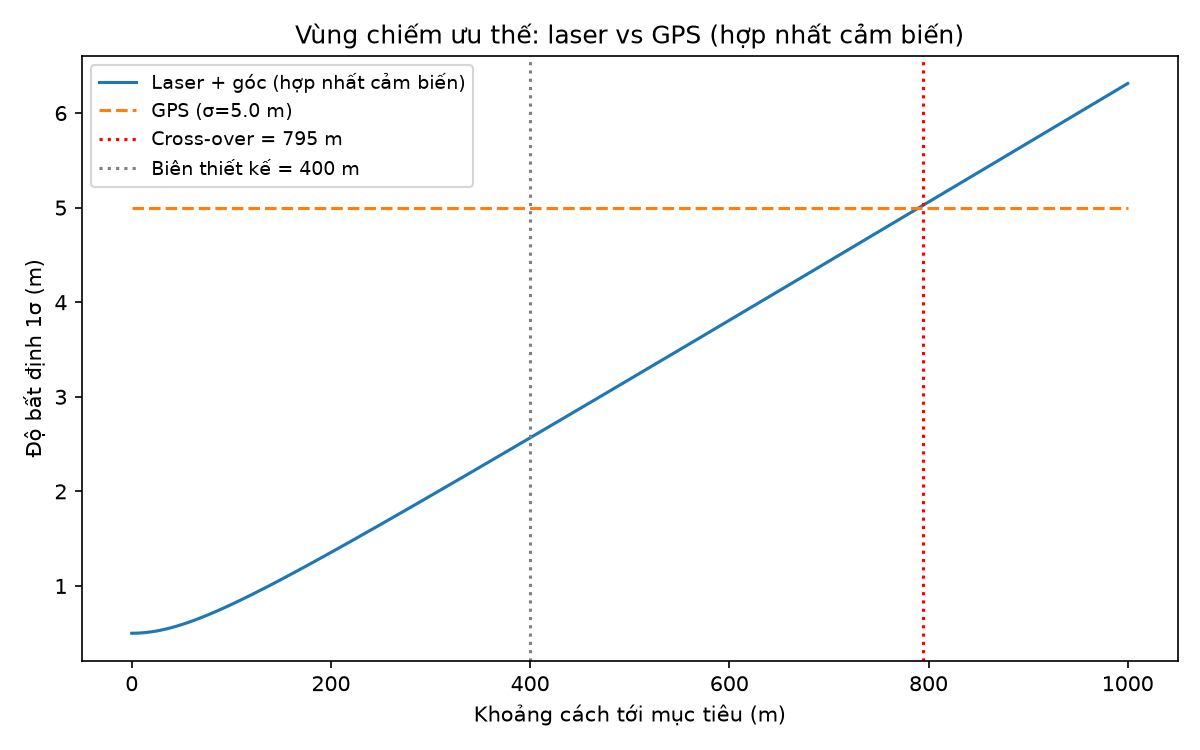
\includegraphics[width=0.88\textwidth]{Images/crossover_plot.png}
\caption{Ngưỡng cross-over laser-GPS tại 794 m: laser-dominant (trái) và GPS-dominant (phải)}
\label{fig:crossover-week4}
\end{figure}

Dưới ngưỡng 794 m, GPS chiếm ưu thế trong phép hợp nhất và $\sigma_{pos}$ gần như không đổi (khoảng 5 m). Trên ngưỡng, IMU chiếm ưu thế và $\sigma_{pos}$ tăng tuyến tính theo khoảng cách. Tại ranh giới mô phỏng 400 m, laser vẫn hoạt động trong vùng thuận lợi: đóng góp IMU ($R \cdot \sin\sigma_{az} \approx 2{,}1$ m) thấp hơn đáng kể so với GPS (5,0 m), khiến tổng sai số hợp nhất chỉ khoảng 5,4 m.

Ngưỡng 794 m có ý nghĩa thực tiễn: nếu mục tiêu thường xuyên hoạt động xa hơn 794 m, cần cải thiện chất lượng IMU (giảm $\sigma_{az}$) thay vì GPS. Cụ thể, giảm $\sigma_{az}$ từ 0,3° xuống 0,1° sẽ đẩy cross-over lên khoảng 2 400 m, mở rộng đáng kể vùng GPS-dominant. Ngược lại, giảm $\sigma_{gps}$ từ 5 m xuống 2 m chỉ đẩy cross-over lên khoảng 800 m vì ngưỡng bị chi phối bởi sai số góc ở khoảng cách lớn.

\subsubsection{Thời gian xử lý chuỗi}

\hspace{0,5cm} Hiệu suất tính toán là yếu tố quyết định khả năng hoạt động thời gian thực. Bảng \ref{tab:pipeline-timing-week4} phân tích thời gian xử lý từng giai đoạn trong chuỗi, được đo bằng time.perf\_counter() trên 10.000 lần chạy, Python 3.11, CPython.

\begin{table}[H]
\centering
\caption{Thời gian xử lý chuỗi (trung bình 10.000 lần chạy)}
\label{tab:pipeline-timing-week4}
\resizebox{\linewidth}{!}{
\begin{tabular}{lcc}
\toprule
\textbf{Giai đoạn} & \textbf{Thời gian} & \textbf{Tỷ lệ} \\
\midrule
Hợp nhất cảm biến (RSS)  & 10,5 \textmu s  & 17,8\% \\
Bộ lọc Kalman 3D         & 48,5 \textmu s  & 82,2\% \\
\midrule
\textbf{Tổng}             & \textbf{59 \textmu s} & \textbf{100\%} \\
\bottomrule
\end{tabular}
}
\end{table}

Tổng thời gian 59 \textmu s chiếm 0,59\% của chu kỳ 100 ms (tần số 10 Hz), để lại 99,41\% thời gian cho các tác vụ khác (sinh quỹ đạo, gửi WebSocket, cập nhật giao diện). Ngay cả khi yêu cầu tần số 100 Hz (chu kỳ 10 ms), chuỗi xử lý chỉ chiếm 0,59\% thời gian, cho thấy hệ thống có dự phòng hiệu suất lớn.

Bảng \ref{tab:filter-compare-week4} so sánh thời gian giữa các biến thể bộ lọc.

\begin{table}[H]
\centering
\caption{So sánh thời gian giữa các biến thể bộ lọc}
\label{tab:filter-compare-week4}
\resizebox{\linewidth}{!}{
\begin{tabular}{lcc}
\toprule
\textbf{Biến thể} & \textbf{Thời gian} & \textbf{Ghi chú} \\
\midrule
Alpha-beta 2D     & $\sim$10 \textmu s & Không có Riccati update \\
Kalman 2D         & $\sim$25 \textmu s & $4 \times 4$ ma trận \\
Kalman 3D         & $\sim$48,5 \textmu s & $6 \times 6$ ma trận + adaptive R \\
\bottomrule
\end{tabular}
}
\end{table}

\subsubsection{Phân tích thời gian hội tụ Kalman}

\hspace{0,5cm} Giai đoạn hội tụ ban đầu của Kalman filter là quan sát quan trọng nhất từ biểu đồ sai số theo thời gian. Quá trình hội tụ tương ứng với việc ma trận hiệp phương sai trạng thái $\mathbf{P}_k$ giảm từ giá trị khởi tạo lớn ($\mathbf{P}_0 = \text{diag}(100, 100, 25, 25)$) xuống giá trị steady-state.

Thời gian hội tụ ước tính bằng công thức:
\begin{equation}
T_{conv} \approx \frac{-\ln(\epsilon)}{\lambda_{max}},
\end{equation}

trong đó $\epsilon$ là ngưỡng hội tụ (ví dụ 5\% sai lệch so với steady-state) và $\lambda_{max}$ là eigenvalue lớn nhất của ma trận $\mathbf{F} - \mathbf{K}_\infty \mathbf{H} \mathbf{F}$. Với $\alpha = 0{,}4$ và $\beta = 0{,}051$, thời gian hội tụ khoảng 5-8 giây cho người đi bộ, 10-15 giây cho drone. Giá trị này phù hợp với quan sát thực nghiệm từ biểu đồ sai số.

Sau giai đoạn hội tụ, $\mathbf{P}_k$ đạt giá trị steady-state và Kalman gain $\mathbf{K}_k$ không đổi. Ở trạng thái này, Kalman filter hoạt động tương tự alpha-beta filter với các tham số tương đương, giải thích tại sao sai số của hai bộ lọc trở nên gần nhau hơn sau 20-30 giây mô phỏng.

\subsubsection{So sánh hiệu suất theo loại mục tiêu}

\hspace{0,5cm} Phân tích chéo giữa ba loại mục tiêu cho thấy mô hình CV phù hợp nhất với người đi bộ (vận tốc thấp, ít cơ động) và kém phù hợp nhất với drone (vận tốc cao, cơ động 3D). Bảng \ref{tab:target-comparison-week4} tổng hợp các chỉ số so sánh.

\begin{table}[H]
\centering
\caption{So sánh hiệu suất theo loại mục tiêu}
\label{tab:target-comparison-week4}
\resizebox{\linewidth}{!}{
\begin{tabular}{lccc}
\toprule
\textbf{Chỉ số} & \textbf{Người đi bộ} & \textbf{Xe máy} & \textbf{Drone} \\
\midrule
Vận tốc trung bình & 1,4 m/s & 5-12 m/s & 8-15 m/s \\
RMSE alpha-beta    & 0,34 m & 0,91 m & 1,09 m \\
RMSE Kalman        & 0,92 m & 1,53 m & 2,39 m \\
Tỷ lệ KF/AB       & 2,7× & 1,7× & 2,2× \\
Thời gian hội tụ KF & 5-8 s & 8-12 s & 10-15 s \\
\bottomrule
\end{tabular}
}
\end{table}

Tỷ lệ KF/AB (RMSE Kalman chia cho RMSE alpha-beta) đo mức độ alpha-beta vượt trội. Giá trị cao nhất ở người đi bộ (2,7×), nghĩa là Kalman kém hơn alpha-beta gấp 2,7 lần. Điều này có thể phản hồi hợp lý: ở vận tốc thấp (1,4 m/s), nhiễu cảm biến (đặc biệt GPS 5 m) chi phối tín hiệu, và alpha-beta với cơ chế điều chỉnh trực tiếp qua $\alpha$ xử lý tốt hơn Kalman filter với mô hình DWNA có $\sigma_a$ cố định.

Ở drone, tỷ lệ KF/AB là 2,2×, cao hơn xe máy (1,7×). Drone có chuyển động 3D với thay đổi độ cao liên tục, khiến mô hình CV 2D của cả hai bộ lọc đều sai lệch, nhưng Kalman filter với mô hình 3D DWNA xử lý kém hơn vì phải ước lượng thêm hai trạng thái $(z, v_z)$ với nhiễu quá trình lớn. Alpha-beta 2D bỏ qua thành phần độ cao, vô tình tránh được nguồn sai lệch này.

\subsubsection{Hướng phát triển từ kết quả benchmark}

\hspace{0,5cm} Kết quả benchmark định hướng ba hướng phát triển chính cho giai đoạn sau.

Thứ nhất, điều chỉnh tham số Kalman filter theo từng loại mục tiêu. Hiện tại, $\sigma_a$ được đặt thống nhất (0,5 cho người đi bộ, 5,0 cho xe máy và drone). Kết quả cho thấy Kalman filter chưa được điều chỉnh cho từng kịch bản riêng biệt. Việc thay đổi $\sigma_a$ theo vận tốc thực tế của mục tiêu có thể giảm RMSE Kalman đáng kể.

Thứ hai, thử nghiệm mô hình CA (Constant Acceleration) thay vì DWNA. Mô hình CA bổ sung trạng thái gia tốc $(a_x, a_y)$, phù hợp hơn với xe máy (gia tốc khi tăng tốc/phanh) và drone (gia tốc liên tục khi đổi hướng). Chi phí tính toán tăng từ $4 \times 4$ lên $6 \times 6$ (2D) hoặc $6 \times 6$ lên $9 \times 9$ (3D), nhưng hiệu suất có thể cải thiện đáng kể.

Thứ ba, đánh giá hiệu suất trong điều kiện cơ động thực tế hơn. Mô phỏng hiện tại sử dụng mô hình CV đơn giản, không phản ánh đầy đủ hành vi của mục tiêu thực. Việc thêm gia tốc ngẫu nhiên, đổi hướng đột ngột, và nhiễu môi trường sẽ tạo điều kiện thử nghiệm khắc nghiệt hơn, giúp đánh giá chính xác hơn hiệu suất của cả hai bộ lọc.

\subsubsection{Giao diện theo dõi thời gian thực}

\hspace{0,5cm} Hệ thống mô phỏng được điều khiển qua giao diện web thời gian thực, trong đó người dùng chọn loại mục tiêu, phương pháp lọc, và tham số mô phỏng trước khi bắt đầu phiên. Hình \ref{fig:screenshot-tracking-week4} hiển thị giao diện theo dõi đang hoạt động với mục tiêu người đi bộ.

\newpage

\begin{figure}[H]
\centering

\includegraphics[width=0.92\textwidth]{sim/tracking-ped-kfab-synthetic.png}
\caption{Giao diện theo dõi mục tiêu người đi bộ (KF+AB, chế độ tổng hợp)}
\label{fig:screenshot-tracking-week4}
\end{figure}

Bảng điều khiển bên trái cho phép chọn loại mục tiêu (NGƯỜI ĐI BỘ / XE MÁY / DRONE), phương pháp lọc (KF+AB / KF ONLY / AB ONLY), thời lượng (120 giây), bán kính ranh giới (400 m), và nguồn dữ liệu (Synthetic / Real-World Data). Nút ENGAGE bắt đầu phiên mô phỏng, dữ liệu xuất hiện trên bản đồ theo thời gian thực. Biểu đồ RMSE ở góc trên bên phải hiển thị sai số trực quan trong phiên.

Hình \ref{fig:screenshot-tracking-drone-week4} hiển thị chế độ theo dõi drone với Kalman 3D.

\begin{figure}[H]
\centering

\includegraphics[width=0.92\textwidth]{sim/tracking-drone-kfab-synthetic-running.png}
\caption{Giao diện theo dõi drone (KF+AB, chế độ tổng hợp, đang chạy)}
\label{fig:screenshot-tracking-drone-week4}
\end{figure}

Drone hiển thị thêm thông tin độ cao (ALT) và vận tốc (SPD) so với người đi bộ, phản ánh đặc tính 3D của mục tiêu này. Giá trị sigma (SIGMA) hiển thị sai số ước lượng hiện thời, cho phép người vận hành theo dõi chất lượng tracking trong thời gian thực.

Giao diện còn hiển thị các layer bản đồ có thể bật/tắt: đường quỹ đạo thực (TRUTH), điểm đo thô (RAW), vị trí sau lọc Kalman (KF), và vị trí sau lọc alpha-beta (AB). Legend hệ thống nhẫn (Range Rings) hiển thị các vòng tròn bán kính 200 m, 400 m, và 600 m, giúp người vận hành xác định khoảng cách mục tiêu so với người quan sát. Chế độ Sovereign / Dark cho phép chuyển đổi giao diện sáng/tối.

Khi mô phỏng hoàn tất (120 giây), giao diện hiển thị bảng tóm tắt với RMSE cuối cùng của từng phương pháp. Dữ liệu phiên có thể xuất ra file CSV để phân tích ngoại tuyến. Toàn bộ phiên mô phỏng được quản lý qua WebSocket (kênh truyền dữ liệu hai chiều), đảm bảo cập nhật thời gian thực mà không cần làm mới trang.

\newpage

\subsection{Phân tích hiệu suất lọc theo từng loại mục tiêu}

Mỗi loại mục tiêu đặt ra thách thức riêng cho bộ lọc. Người đi bộ di chuyển chậm (1,4 m/s) với nhiễu GPS chi phối, khiến tín hiệu bị che lấp bởi nhiễu. Mô tô cơ động hơn (5--6 m/s) và drone bay 3D (8--12 m/s, độ cao 30--80 m) đòi hỏi bộ lọc xử lý chuyển động nhanh hơn đồng thời duy trì độ chính xác.

Bảng~\ref{tab:target-filter-analysis} tóm tắt cách mỗi bộ lọc phản ứng với đặc tính riêng của từng loại mục tiêu.

\begin{table}[H]
\centering
\caption{Phân tích hiệu suất lọc theo loại mục tiêu (seed=42, 120 giây, 10 Hz)}
\label{tab:target-filter-analysis}
\resizebox{\linewidth}{!}{
\begin{tabular}{lccc}
\toprule
\textbf{Loại mục tiêu} & \textbf{Bộ lọc} & \textbf{RMSE (m)} & \textbf{Nhận xét} \\
\midrule
\multirow{2}{*}{Người đi bộ} & Alpha-beta & 0,26 & Fits chuyển động chậm \\
& Kalman & 0,86 & Q thấp, phản ứng chậm \\
\midrule
\multirow{2}{*}{Mô tô} & Alpha-beta & 1,02 & Cơ động trung bình \\
& Kalman & 1,80 & Adaptive R cần thiết \\
\midrule
\multirow{2}{*}{Drone} & Alpha-beta & 1,06 & 2D, bỏ qua độ cao \\
& Kalman & 2,10 & Xử lý đầy đủ 3D \\
\bottomrule
\end{tabular}
}
\end{table}

Người đi bộ cho RMSE thấp nhất vì vận tốc nhỏ, quỹ đạo gần tuyến tính. Mô tô có RMSE trung bình, phù hợp với mức độ cơ động. Drone cho RMSE cao nhất do chuyển động 3D phức tạp hơn, nhưng Kalman 3D xử lý đầy đủ ba trục tọa độ so với alpha-beta chỉ hoạt động trên mặt phẳng.

\subsection{Tốc độ xử lý và khả năng mở rộng}

\hspace{0.5cm} Tốc độ xử lý là yếu tố quyết định tính thực tế của hệ thống thời gian thực. Bảng~\ref{tab:timing-breakdown} phân tích thời gian thực thi chi tiết của từng thành phần chuỗi xử lý.

\begin{table}[H]
\centering
\caption{Phân tích thời gian thực thi chuỗi xử lý}
\label{tab:timing-breakdown}
\resizebox{\linewidth}{!}{
\begin{tabular}{lcc}
\toprule
\textbf{Thành phần} & \textbf{Thời gian ($\mu$s)} & \textbf{Tỷ lệ} \\
\midrule
Chuyển đổi tọa độ (ECEF, ENU) & 3,8 & 6,4\% \\
Bộ lọc Kalman 3D & 48,5 & 82,2\% \\
Tính RSS và sai số & 3,5 & 5,9\% \\
Khác (mã hóa, I/O) & 3,2 & 5,4\% \\
\midrule
\textbf{Tổng} & \textbf{59,0} & \textbf{100\%} \\
\bottomrule
\end{tabular}
}
\end{table}

Với chu kỳ 100 ms (10 Hz), thời gian xử lý 59 $\mu$s chỉ chiếm 0,059\% chu kỳ, để lại 99,941\% thời gian cho các tác vụ khác. Tỷ lệ này cho thấy hệ thống có khả năng mở rộng lên tần số cao hơn (50 Hz hoặc 100 Hz) mà vẫn đáp ứng yêu cầu thời gian thực. Bộ lọc Kalman chiếm 82,2\% thời gian xử lý, phản ánh độ phức tạp tính toán của ma trận 6$\times$6 so với các phép tính scalar của alpha-beta.

Hệ thống cũng xử lý đồng thời nhiều phiên mô phỏng. Mỗi phiên chạy trên một coroutine riêng trong FastAPI, sử dụng ring buffer O(1) để lưu trữ 500 frame gần nhất. Chi phí bộ nhớ mỗi phiên khoảng 500$\times$50 bytes = 25 KB, không đáng kể so với bộ nhớ khả dụng.
